\documentclass[]{article}
\usepackage{lmodern}
\usepackage{setspace}
\setstretch{2}
\usepackage{amssymb,amsmath}
\usepackage{ifxetex,ifluatex}
\usepackage{fixltx2e} % provides \textsubscript
\ifnum 0\ifxetex 1\fi\ifluatex 1\fi=0 % if pdftex
  \usepackage[T1]{fontenc}
  \usepackage[utf8]{inputenc}
\else % if luatex or xelatex
  \ifxetex
    \usepackage{mathspec}
  \else
    \usepackage{fontspec}
  \fi
  \defaultfontfeatures{Ligatures=TeX,Scale=MatchLowercase}
\fi
% use upquote if available, for straight quotes in verbatim environments
\IfFileExists{upquote.sty}{\usepackage{upquote}}{}
% use microtype if available
\IfFileExists{microtype.sty}{%
\usepackage{microtype}
\UseMicrotypeSet[protrusion]{basicmath} % disable protrusion for tt fonts
}{}
\usepackage[margin=1in]{geometry}
\usepackage{hyperref}
\hypersetup{unicode=true,
            pdfborder={0 0 0},
            breaklinks=true}
\urlstyle{same}  % don't use monospace font for urls
\usepackage{graphicx,grffile}
\makeatletter
\def\maxwidth{\ifdim\Gin@nat@width>\linewidth\linewidth\else\Gin@nat@width\fi}
\def\maxheight{\ifdim\Gin@nat@height>\textheight\textheight\else\Gin@nat@height\fi}
\makeatother
% Scale images if necessary, so that they will not overflow the page
% margins by default, and it is still possible to overwrite the defaults
% using explicit options in \includegraphics[width, height, ...]{}
\setkeys{Gin}{width=\maxwidth,height=\maxheight,keepaspectratio}
\IfFileExists{parskip.sty}{%
\usepackage{parskip}
}{% else
\setlength{\parindent}{0pt}
\setlength{\parskip}{6pt plus 2pt minus 1pt}
}
\setlength{\emergencystretch}{3em}  % prevent overfull lines
\providecommand{\tightlist}{%
  \setlength{\itemsep}{0pt}\setlength{\parskip}{0pt}}
\setcounter{secnumdepth}{0}
% Redefines (sub)paragraphs to behave more like sections
\ifx\paragraph\undefined\else
\let\oldparagraph\paragraph
\renewcommand{\paragraph}[1]{\oldparagraph{#1}\mbox{}}
\fi
\ifx\subparagraph\undefined\else
\let\oldsubparagraph\subparagraph
\renewcommand{\subparagraph}[1]{\oldsubparagraph{#1}\mbox{}}
\fi

%%% Use protect on footnotes to avoid problems with footnotes in titles
\let\rmarkdownfootnote\footnote%
\def\footnote{\protect\rmarkdownfootnote}

%%% Change title format to be more compact
\usepackage{titling}

% Create subtitle command for use in maketitle
\newcommand{\subtitle}[1]{
  \posttitle{
    \begin{center}\large#1\end{center}
    }
}

\setlength{\droptitle}{-2em}
  \title{}
  \pretitle{\vspace{\droptitle}}
  \posttitle{}
  \author{}
  \preauthor{}\postauthor{}
  \date{}
  \predate{}\postdate{}

\fontsize{12}{20}
\usepackage{lineno}
\linenumbers
\linenumberfont
\renewcommand\linenumberfont{\normalfont\small\sffamily}
\pagenumbering{gobble}

\begin{document}

\linenumbers[787]

\subsection{Figure legends}\label{figure-legends}

Fig. 1. Bomb carbon dating age validation studies on shark and ray
populations showing validated, uncertain and underestimated ages,
ordered by increasing maximum age. The number of samples in each study
is given at the end of each bar.

Fig. 2. Chemical marking age validation studies on shark and ray
populations showing validated, uncertain and underestimated ages,
ordered by increasing maximum age. The number of samples in each study
is given at the end of each bar. * the age of some individuals was
underestimated, but their revised age did not exceed that of the oldest
individual aged.

Fig. 3. Occurrence and magnitude of age underestimation in 61
individuals from 10 bomb carbon dating age validation studies. (a) Plot
of relative age (Age/\(A_{Max}\)) against relative length
(Length/\(L_\infty\)), size of points denotes the discrepancy between
true and apparent age (\(\Delta\) Age). (b) and (c) are logistic
regression analyses modelling the probability of age underestimation as
a function of relative length and age, respectively. White points in (b)
and (c) were excluded from statistical analysis. NEP, northeast Pacific;
NWA, northwest Atlantic; SA, South Africa.

Fig. 4. Hypothesised effects and implications of age underestimation on
growth and mortality, illustrated with simulated data for New Zealand
porbeagle sharks (Francis \emph{et al} 2007). (a) The growth curve
asymptote is effectively truncated when older individuals are
under-aged, and this may result in a steeper curve with biased
parameters. (b) Assuming age underestimation is a function of length,
faster-growing individuals will be affected at a younger age than
slower-growing individuals. (c) The apparent loss of age structure due
to age underestimation may be inadvertently attributed to or
indistinguishable from the effects of fishing. (d) Comparison of true
\(A_{Max}\) = 65 years versus apparent \(A_{Max}\) = 35 years in
population projection from a simple, density-independent demographic
analysis assuming Hoenig mortality (see Supplementary Material for
additional information). \newpage

\subsection{Figures}\label{figures}

\nolinenumbers

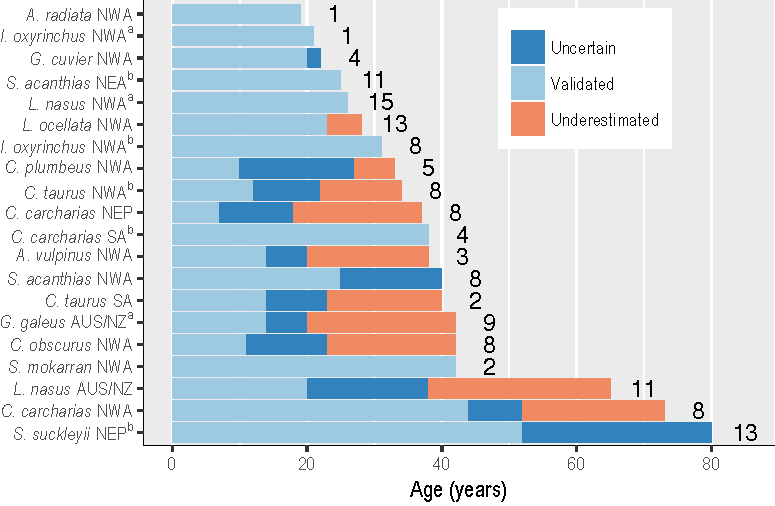
\includegraphics{/Users/alharry/Documents/Manuscripts/age-underestimation/reports/Figures_files/figure-latex/fig1-1.pdf}

Fig 1.\\
\newpage
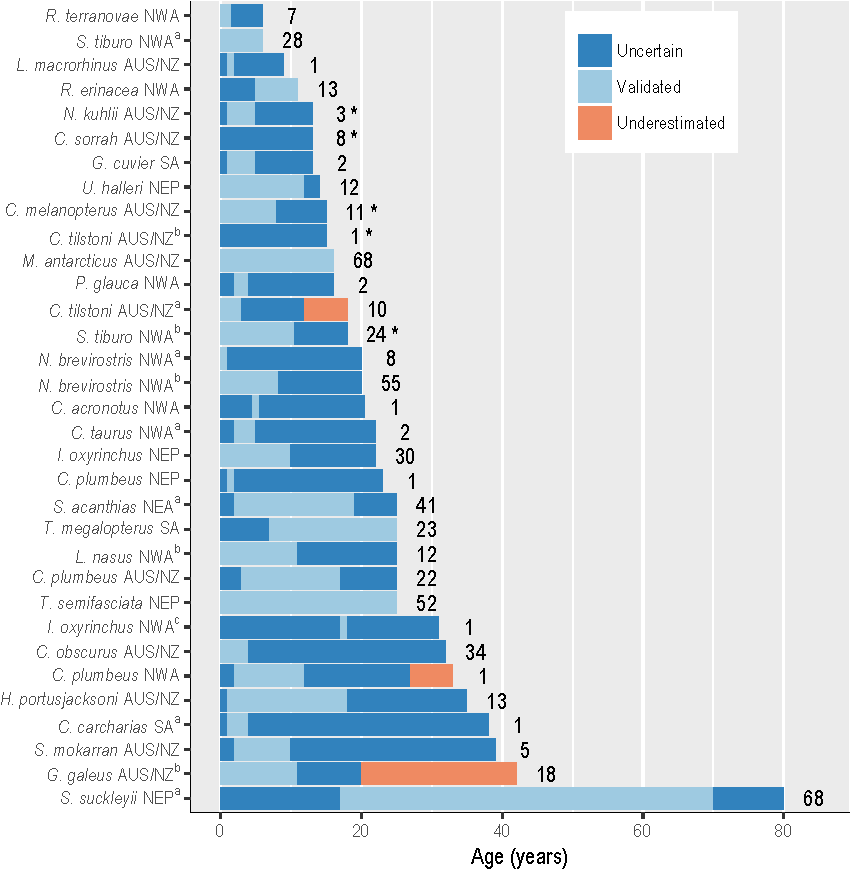
\includegraphics{/Users/alharry/Documents/Manuscripts/age-underestimation/reports/Figures_files/figure-latex/fig2-1.pdf}

Fig 2.\\
\newpage
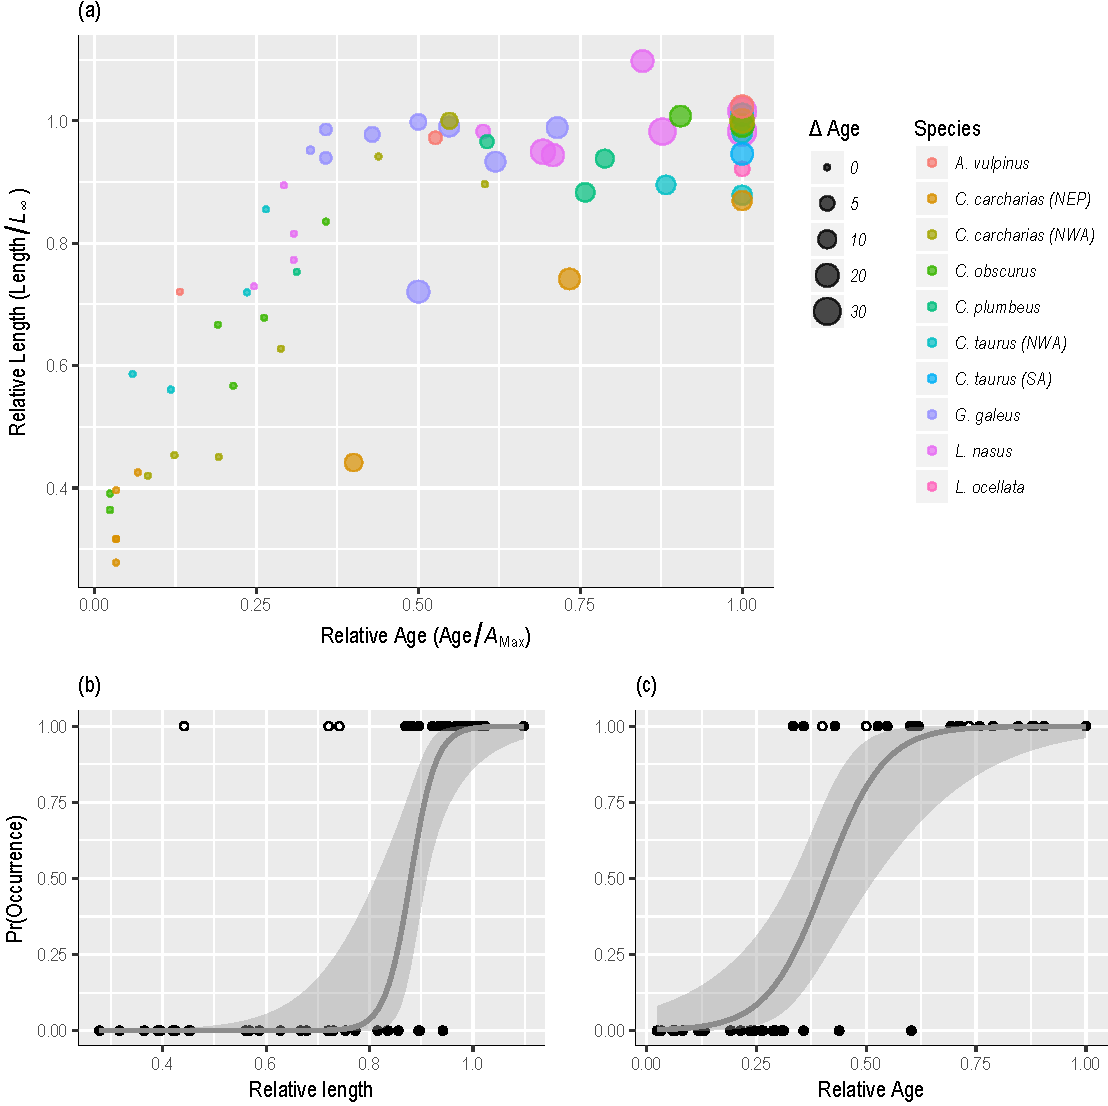
\includegraphics{/Users/alharry/Documents/Manuscripts/age-underestimation/reports/Figures_files/figure-latex/fig3-1.pdf}

Fig 3.\\
\newpage
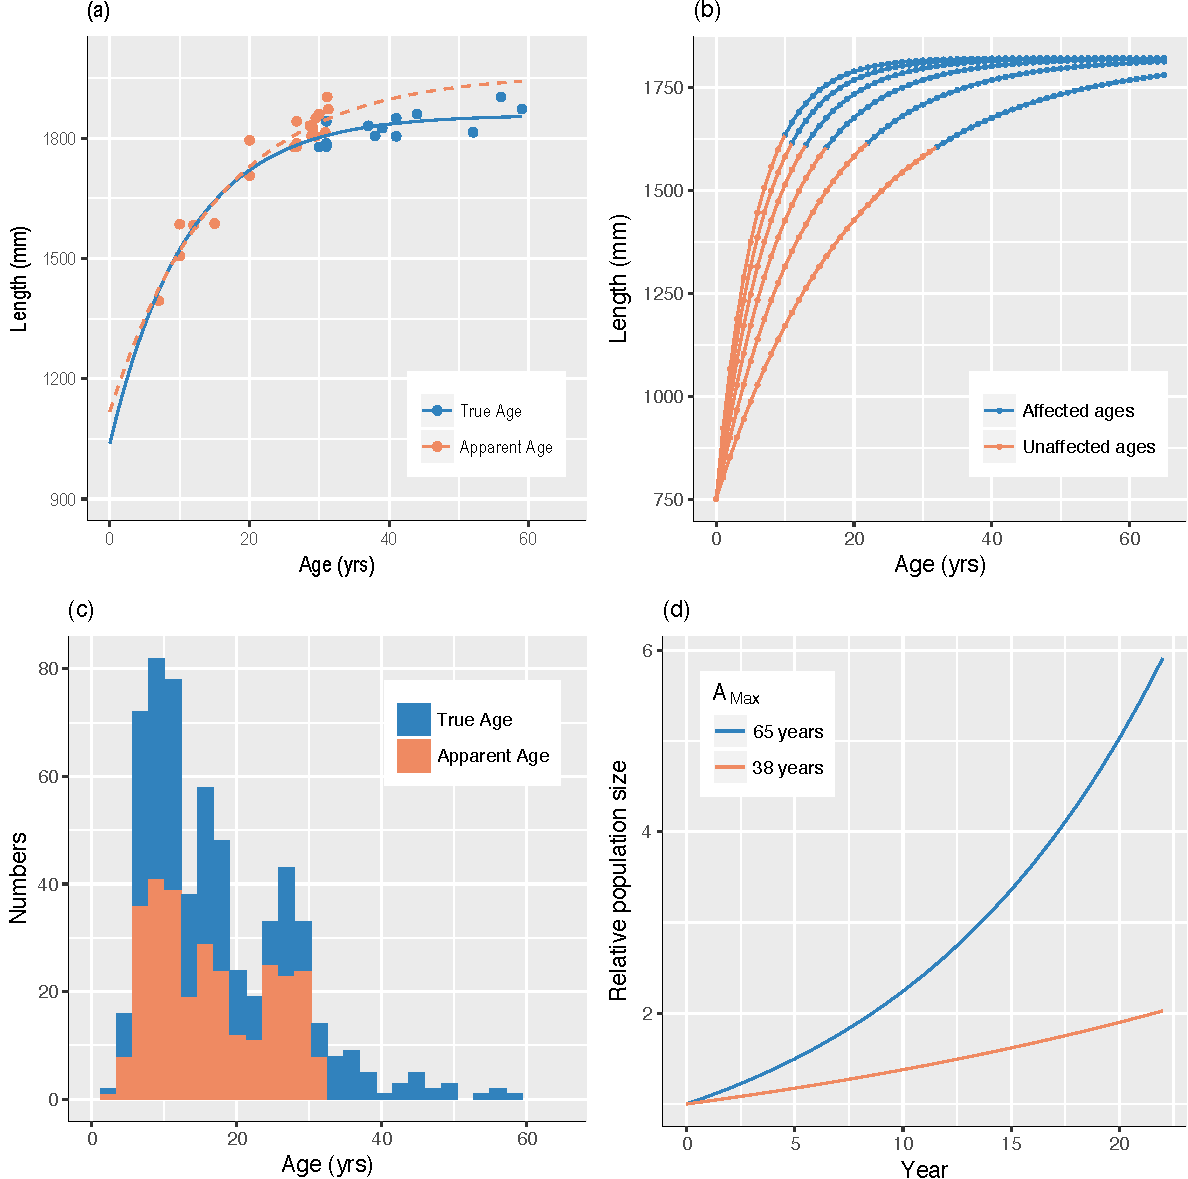
\includegraphics{/Users/alharry/Documents/Manuscripts/age-underestimation/reports/Figures_files/figure-latex/fig4-1.pdf}

Fig 4.


\end{document}
